\documentclass[12pt,a4paper]{article}
\usepackage[utf8]{inputenc}
\usepackage[T1]{fontenc}
\usepackage{titling}
\usepackage{amsfonts}
\usepackage{amssymb}
\usepackage{tcolorbox}
\usepackage{mdframed}
\usepackage{graphicx}
\usepackage{wrapfig}
\usepackage{libertine}
\usepackage{tikzpagenodes}
\usepackage{float}
\usepackage{amsfonts}
\usepackage[top=1in, bottom=1.5in, left=1in, right=1in]{geometry}
\renewcommand{\contentsname}{Sadržaj}

\setlength{\droptitle}{-8em}




\title{\vspace{-2.3cm}\Large \textsc{univerzitet u novom sadu
\\prirodno-matematički fakultet
\\departman za
\\matematiku i informatiku}
\vspace{5em} 
\\ \textbf{Remzijevi brojevi}
\\ - \large seminarski rad -
\vspace{1em} }


\graphicspath{ {/hdd/seminarski/GeogebraSlike//} }

\begin{document}

	\begin{figure}[]
	\centering
	\advance\leftskip-14cm
	
\includegraphics[scale=0.3]{logo1.png}
	\end{figure}
	

	\begin{figure}[]
	\vspace{-3.4cm}
	\centering
	\advance\leftskip14cm
	
\includegraphics[scale=0.3]{logo2.png}
	\end{figure}

	\author{
  	Renea Mošo\\
  	\texttt{}
  	\and
  	Nikola Obradović\\
  	\texttt{}
  	\and
  	Nikola Pešić
	}	
	\date{}
	
	
	\maketitle
	
	\thispagestyle{empty}
	
	\newpage
	
	
	\tableofcontents
	\newpage
	
	\section{Uvod u Remzijevu teoriju}
	Obrad
	\newpage
	
	
	\section{Remzijevi brojevi}
	\vspace{1em}
	{\fontsize{12pt}{12pt}\textbf{Definicija}}
	\vspace{0.5em}	
	\\
	Remzijev broj $R(l_{1}, l_{2})$ je najmanje $n \in \mathbb{N}$ \textbackslash {} $\left\lbrace 0\right\rbrace $ takvo da $n\rightarrow(l_{1}, l_{2})$.
	
	
	\vspace{1em}
	{\noindent\fontsize{12pt}{12pt}\textbf{Primer}}
	\vspace{0.5em}
	\\	
	Pronađimo $R(3,3)$ :
	\\Počnimo od broja 6. Dokazaćemo da je $6 \rightarrow (3, 3)$. Uočimo čvor A. Po Dirihleovom principu bar 3 od 5 veza čvora A sa ostalim čvorovima mora biti obojeno istom bojom. 
	\begin{figure}[h]
	\centering
	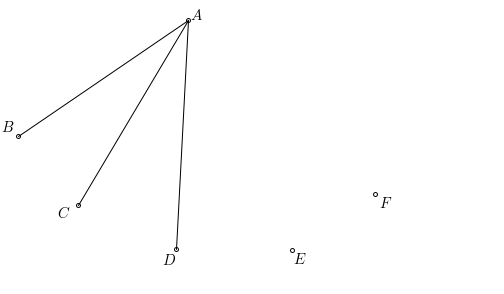
\includegraphics[scale=2.3]{r33.png}
	\end{figure}
	
	\noindent Na slici su grane jedne boje obojene u crno, dok su ostale bele (ne vide se).
	Neka su, bez umanjenja opštosti, grane čvora A koje su incidentne sa čvorovima B, C i D obojene istom bojom (crnom). Sada postoje dve mogućnosti: 
	\vspace{1em}
	\\
	$1^\circ$ Sve grane koje povezuju čvorove B, C i D su obojene belom bojom Tada čvorovi B, C, i D obrazuju kompletan graf reda 3 obojen belom bojom.
	\vspace{0.5em}
	\\
	$2^\circ$ Bar jedna od grana koje povezuju čvorove B, C i D je obojena crnom bojom. Bez umanjenja opštosti, neka je to grana koja povezuje B i C. Tada čvorovi A, B i C sačinjavaju kompletan graf reda 3 obojen crnom bojom.
	\vspace{0.5em}
	\\Dokazali smo da je $6 \rightarrow (3, 3)$, a sada još treba dokazati da ne važi $5 \rightarrow (3, 3)$. Za to je dovoljno da pronađemo kontra primer bojenja u kojem uslov nije ispunjen:
	\begin{figure}[h]
	\centering
	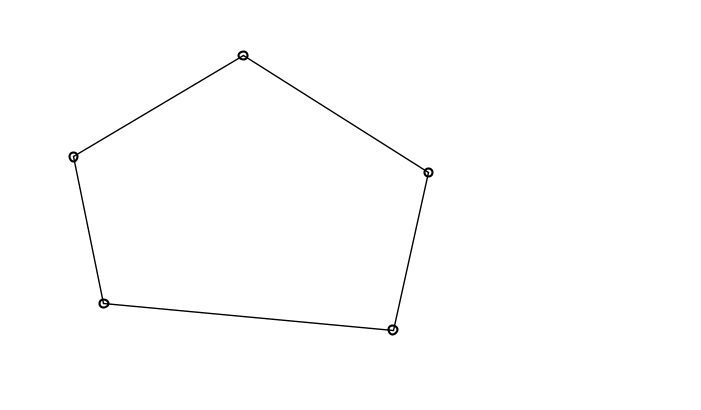
\includegraphics[scale=1.3]{r33kp.png}
	\end{figure}
	
	Dakle, $R(3,3)=6$ .	
	
	\newpage
	
	{\noindent\fontsize{12pt}{12pt}\textbf{Teorema 2.1}}
	\vspace{0.5em}	
	\\
	(1) {} {} $R(1, m) = R(m, 1) = 1$\\
	(2) {} {} $R(2, m) = R(m, 2) = m$\\
	(3) {} {} $R(l_{1}, l_{2}) = R(l_{2}, l_{1})$\\
	(4) {} {} $l \leq r \Rightarrow R(l, m) \leq R(r, m)$\\
	
	{\noindent\fontsize{12pt}{12pt}\textbf{Dokaz 2.1}}
	
	\vspace{0.5em}
	
	\noindent(1) {} {} U grafu reda 1 uvek postoji kompletan podgraf reda 1 čije su sve grane obojene istom bojom, stoga broj $m$ ne utiče na $R(1, m)$.
	\vspace{0.5em} 	\\
	\noindent(2) {} {} U grafu reda m, ili su sve grane obojene jednom bojom, ili postoji bar 1 grana koje je obojena različitom bojom od ostalih. Ako su sve grane obojene jednom bojom imamo kompletan podgraf reda $m$ čije su sve grane obojene istom bojom. Sa druge strane, ako postoji grana koja je obojena različitom bojom, čvorovi sa kojima je ta grana incidentna indukuju podgraf reda $2$ čije su sve grane obojene jednom bojom.
	\vspace{0.5em} \\
	\noindent(3) {} {} Redosled $l_{1}$ i $l_{2}$ ne utiče na $R(l_{1}, l_{2})$ jer sve za svako bojenje grana boje mogu obrnuti.
	\vspace{0.5em} \\
	\noindent(4) {} {} Pretpostavimo suprotno: $l \leq r \Rightarrow R(l, m) > R(r, m)$. Kako je $R(r, m) \rightarrow (r,m)$ i  $l \leq r$, sledi $R(r, m) \rightarrow (l, m)$, ali onda $R(l, m)$ nije Remzijev broj za $(l,m)$ jer postoji broj manji od njega koji je dovoljan za $(l, m)$. Kontradikcija.
	\vspace{1.5em}
	
	{\noindent\fontsize{12pt}{12pt}\textbf{Teorema 2.2}}
	\vspace{0.5em}	
	\\
	Za sve $m,n \geq 2$ važi
	\[R(m,n) \leq {m+n-2\choose m-1} = {m+n-2\choose n-1}\]
	\vspace{1em}
	{\noindent\fontsize{12pt}{12pt}\textbf{Dokaz 2.2}}	\vspace{-0.5em}
	\\
	\noindent Ovu teoremu dokazaćemo indukcijom.\\
	Baza indukcije:\\
	\[R(1,2) = R(2,1) = 1 \leq {1+2-2\choose 1-0}={1\choose 0}=1\]\\
	Indukcijska hipoteza:
	Neka tvrđenje važi za sve $(p,q)<(m,n)$.\\
	Indukcijski korak: po indukcijskoj hipotezi važi 
	\[R(m-1, n) \leq {m+n-3\choose m-2} \quad tj. \quad {m+n-3\choose m-2}\rightarrow (m-1, n)\] 
	\[R(m, n-1) \leq {m+n-3\choose m-1} \quad tj. \quad {m+n-3\choose m-1}\rightarrow (m, n-1)\]
	
	Sada iz Paskalove formule i Teoreme 1.? sledi 
	\[{m+n-3\choose m-2}+{m+n-3\choose m-1}={m+n-2\choose m-1}\rightarrow (m,n)\] 
	\\
	\vspace{0.7em} tj. $R(m,n) \leq {m+n-2\choose m-1}$, što je i trebalo dokazati. 
	
	
	\section{Granice remzijevih brojeva}
	Pesic
\end{document}